\documentclass[a4paper,12pt,titlepage]{article}
\usepackage{amsmath} 
\usepackage{amssymb}
\usepackage[nottoc]{tocbibind}
\usepackage{float}
\author{\textit{Jiang Yicheng}\\\textit{515370910224}}
\title{\textbf{VV286\\ Honors Mathematics IV\\
Ordinary Differential Equations\\
		Assignment 1}}
\date{\today}

\usepackage[top=1 in, bottom=1 in, left= 1in, right=1 in]{geometry}
\usepackage{fancyhdr,lastpage}
	\pagestyle{fancy}
	\fancyhf{}
\cfoot{Page \thepage\ of \pageref{LastPage}}
\usepackage{multirow}
\usepackage{gauss}
\usepackage{geometry}
\usepackage{graphicx}
\begin{document}

\maketitle


\section{Exercise 1}
\subsection{}
\begin{figure}[ht]
	\centering
	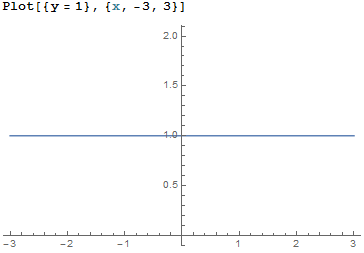
\includegraphics[height=10cm]{1.png}
	\caption{Direction field for $y'=\sqrt{|y|}$}  
\end{figure}

\subsection{}
If $\forall x\in R,y(x)=0$, we can see that this is a solution to the differential equation $y'=\sqrt{|y|}$. For other possible solutions, they can be found through the equation
$$\int^y_0\dfrac{ds}{\sqrt{|s|}}=\int_1^xdt$$ 
we can see that the integral on the left-hand side left-hand side exists for $y$ in a small neighborhood of 0 since
\begin{align*}
\int^y_0\dfrac{ds}{\sqrt{|s|}}=\left\{
\begin{aligned}
\int^y_0\dfrac{ds}{\sqrt{s}},s\geqslant0\\
\int^y_0\dfrac{ds}{\sqrt{-s}},s<0\\
\end{aligned}
\right.
=\left\{\begin{aligned}
&2\sqrt{y},y\geqslant0\\
&-2\sqrt{-y},y<0\\
\end{aligned}
\right.
\end{align*}
So the possible solution except $y=0$ is given by $x-1=\left\{\begin{aligned}
&2\sqrt{y},y\geqslant0\\
&-2\sqrt{-y},y<0\\
\end{aligned}
\right.$, i.e.$y=\left\{\begin{aligned}
&\dfrac{1}{4}(x-1)^2,x\geqslant1\\
&-\dfrac{1}{4}(x-1)^2,x<1\\
\end{aligned}
\right.$

For this function, first we can see that it's differentiable since $\underset{x\nearrow1}{lim}\dfrac{dy}{dx}=0=\underset{x\searrow1}{lim}\dfrac{dy}{dx}$. And for $x\geqslant1$, $y\geqslant0$ and  $y'=\dfrac{1}{2}(x-1)=\sqrt{\dfrac{1}{4}(x-1)^2}=\sqrt{y}$; while for $x<1$, $y<0$ and  $y'=-\dfrac{1}{2}(x-1)=\sqrt{\dfrac{1}{4}(x-1)^2}=\sqrt{-y}$. So $y'=\sqrt{|y|}$ always holds and therefore this is a solution for the differential equation.

To sum up, all solutions of this problem are
\begin{enumerate}
\item $y=0(x\in\mathbb{R})$
\item $y=\left\{\begin{aligned}
&\dfrac{1}{4}(x-1)^2,x\geqslant1\\
&-\dfrac{1}{4}(x-1)^2,x<1\\
\end{aligned}
\right.$
\end{enumerate} 

\section{Exercise 2}
\section{Exercise 3}
\paragraph{Proof:}Since $y_{\xi}(\xi)=0$, then $\forall \xi\in\overline{I}$
\begin{align*}
y'=\dfrac{d}{dx}\int_{x_0}^xf(\xi)y_{\xi}(x)d\xi=y_x(x)f(x)+\int_{x_0}^xf(\xi)y'_{\xi}(x)d\xi=\int_{x_0}^xf(\xi)y'_{\xi}(x)d\xi
\end{align*}

Since $y'_{\xi}(\xi)=0$, then $\forall \xi\in\overline{I}$
\begin{align*}
y''=\dfrac{d}{dx}\int_{x_0}^xf(\xi)y'_{\xi}(x)d\xi=y'_x(x)f(x)+\int_{x_0}^xf(\xi)y''_{\xi}(x)d\xi=\int_{x_0}^xf(\xi)y''_{\xi}(x)d\xi
\end{align*}

So we can see that $\forall n\in\mathbb{N},n\leqslant p-1$, $y^{(n)}=\int_{x_0}^xf(\xi)y^{(n)}_{\xi}(x)d\xi,(y^{(0)}=y)$. Since $y_{\xi}^{(p-1)}(\xi)=\dfrac{1}{a_p(\xi)}$, then
$$y^{(p)}=\dfrac{d}{dx}\int_{x_0}^xf(\xi)y^{(p-1)}_{\xi}(x)d\xi=y^{(p-1)}_x(x)f(x)+\int_{x_0}^xf(\xi)y^{(p)}_{\xi}(x)d\xi=\dfrac{f(x)}{a_p(x)}+\int_{x_0}^xf(\xi)y^{(p)}_{\xi}(x)d\xi$$

 $\forall n\in\mathbb{N},n\leqslant p-1$, $y^{(n)}(x_0)=\int_{x_0}^{x_0}f(\xi)y^{(n)}_{\xi}(x)d\xi=0$, so $y(x)=\int_{x_0}^xf(\xi)y_{\xi}(x)d\xi$ satisfies the
initial condition. Moreover, since $\sum\limits_{n=0}^{p}(a_n(x)y^{(n)}_{\xi}(x))=0$
\begin{align*}
&a_p(x)y^{(p)}+\cdots+a_1(x)y'+a_0(x)y\\
=&a_p(x)(\dfrac{f(x)}{a_p(x)}+\int_{x_0}^xf(\xi)y^{(p)}_{\xi}(x)d\xi)+\sum\limits_{n=0}^{p-1}(a_n(x)\int_{x_0}^xf(\xi)y^{(n)}_{\xi}(x)d\xi)\\
=&f(x)+\sum\limits_{n=0}^{p}(a_n(x)\int_{x_0}^xf(\xi)y^{(n)}_{\xi}(x)d\xi)\\
=&f(x)+\int_{x_0}^xf(\xi)\sum\limits_{n=0}^{p}(a_n(x)y^{(n)}_{\xi}(x))d\xi\\
=&f(x)
\end{align*}
So $y(x)=\int_{x_0}^xf(\xi)y_{\xi}(x)d\xi$ solves $a_p(x)y^{(p)}+\cdots+a_1(x)y'+a_0(x)y=f(x)$.

\section{Exercise 4}
\paragraph{Proof:}Since $y_{hom}$ is a solution of $a_1(x)y'+a_0(x)y=0$,  $a_1(x)y'_{hom}(x)+a_0(x)y_{hom}(x)=0$
\begin{align*}
&a_1(x)y'+a_0(x)y=f(x)\\
\Rightarrow&a_1(x)(\dfrac{d}{dx}(c(x)y_{hom}(x)))+a_0(x)c(x)y_{hom}(x)=f(x)\\
\Rightarrow&a_1(x)c'(x)y_{hom}(x)+c(x)(a_1(x)y'_{hom}(x)+a_0(x)y_{hom}(x))=f(x)\\
\Rightarrow&a_1(x)c'(x)y_{hom}(x)=f(x)\\
\Rightarrow&c'(x)=\dfrac{f(x)}{a_1(x)y_{hom}(x)}\\
\Rightarrow&\int_{x_0}^xc'(\xi)d\xi=\int_{x_0}^x\dfrac{f(\xi)}{a_1(\xi)y_{hom}(\xi)}d\xi\\
\Rightarrow&c(x)=\int_{x_0}^xf(\xi)d\xi(Let\,\,\,c(x_0)=0, and\,\,\,use\,\,\,\forall \xi\in \overline{I} a_1(\xi)y_{hom}(\xi)=1) \\
\Rightarrow&y_{part}(x)=c(x)y_{hom}(x)=y_{hom}(x)\int_{x_0}^xf(\xi)d\xi=\int_{x_0}^xf(\xi)y_{hom}(x)d\xi
\end{align*}
So this differential equation yields the same solution formula as the Duhamel principle.

\section{Exercise 5}
For "Washing of Feet",
$$\lambda y_0=12.6\times 2^{150\div 11}-0.26\times(2^{150\div 11}-1)\approx157134$$
For "Woman Reading Music",
$$\lambda y_0=10.3\times 2^{150\div 11}-0.3\times(2^{150\div 11}-1)\approx127337$$
For "Woman Playing Mandolin",
$$\lambda y_0=8.2\times 2^{150\div 11}-0.17\times(2^{150\div 11}-1)\approx102252$$
All these values are unacceptably large. Thus, "Washing of Feet", "Woman Reading Music" and "Woman playing Mandolin" are forgeries.
\section{Exercise 6}
\subsection{}
According to the question, we have the following differentiable equation:
$$\dfrac{dX}{dt}=k(60-X)(150-X),X(5)=10$$
where k is a constant.

The unique solution of this equation can be obtained from:
$$\int_{10}^X\dfrac{ds}{(60-s)(150-s)}=\int_5^tkdt$$
So $90k(t-5)=\int_{10}^X(\dfrac{1}{60-s}-\dfrac{1}{150-s})ds=ln\dfrac{150-X}{60-X}-ln2.8$. When $t=0, X=0$, so $-450k=ln(2.5/2.8)$. So $X=60-\dfrac{90}{2.8\cdot(25/28)^{(5-t)/5}-1}$
\begin{figure}[ht]
	\centering
	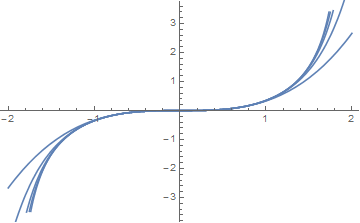
\includegraphics[scale=1]{2.png}
	\caption{The amount of chemical C formed as a function of time}  
\end{figure}

\subsection{}
$$X(20)=60-\dfrac{90}{2.8\cdot(25/28)^{(5-20)/5}-1}\approx29.323g$$
So there are $29.323g$ chemical C formed in 20 minutes.

\subsection{}
$$\underset{t\rightarrow \infty}{lim}X(t)=\underset{t\rightarrow \infty}{lim}60-\dfrac{90}{2.8\cdot(25/28)^{(5-t)/5}-1}=60g$$
So the limiting amount of C as time $t\rightarrow \infty$ is $60g$.

\subsection{}
$$M_A=40-60\times2\div3=0g, M_B=50-60\times1\div3=30g$$
So as time $t\rightarrow \infty$, chemicals A remains $0g$, chemicals B remains $30g$. 



\section{Exercise 7}
\begin{figure}[ht]
	\centering
	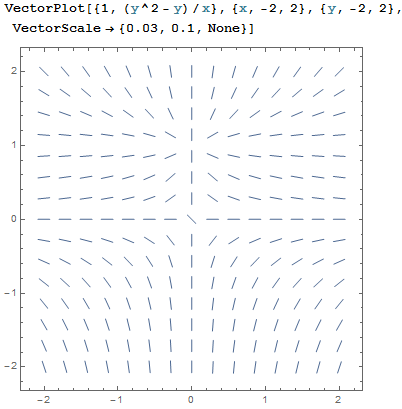
\includegraphics[scale=1]{3.png}
	\caption{The direction field of the equation $xy'=y^2-y$}  
\end{figure}

\subsection{}
The solution that pass through (2,1/4) is $y=\left\{\begin{aligned}
&\dfrac{2}{2-3x},x<0\\
&\dfrac{2}{2+3x},x>0\\
\end{aligned}
\right.$

\subsection{}
The solution that pass through (1/2,1/2) is $y=\left\{\begin{aligned}
&\dfrac{1}{1-2x},x<0\\
&\dfrac{1}{1+2x},x>0\\
\end{aligned}
\right.$

\subsection{}
Since (0,2) doesn't satisfy the differentiable equation, so there is no solution for this situation.

\subsection{}
One solution that pass through (0,1) is $y=1$

\section{Exercise 8}
\subsection{}
\begin{enumerate}
\item $y=-1$ is a solution of the equation $y'=(1+x)(1+y)$
\item If there exists some $x_0$ such that $y(x_0)=y_0\neq-1$, then the solution can be found by 
$$\int_{y_0}^y\dfrac{ds}{1+s}=\int_{x_0}^x1+tdt$$
So 
$$t+\dfrac{1}{2}t^2|^x_{x_0}=ln(1+s)|_{y_0}^y\Rightarrow y=(1+y_0)e^{0.5x^2+x-x_0-0.5x_0^2}-1$$
\end{enumerate}
To sum up, the general solution to $y'=(1+x)(1+y)$ with initial value $y(x_0)=y_0$ is $$y=(1+y_0)e^{0.5x^2+x-x_0-0.5x_0^2}-1$$.

\subsection{}
The solution to $y'=e^{x+y+3}$ can be found by 
$$\int_{y_0}^y\dfrac{ds}{e^s}=\int_{x_0}^xe^{t+3}dt$$
So 
$$e^{t+3}|^x_{x_0}=-e^{-s}|_{y_0}^y\Rightarrow y=-ln(e^{-y_0}-e^{x+3}+e^{x_0+3})$$

To sum up, the general solution to $y'=e^{x+y+3}$ with initial value $y(x_0)=y_0$ is $$y=-ln(e^{-y_0}+e^{x_0+3}-e^{x+3})$$.




\end{document}